\chapter{Discussion}
\label{chap:discussion}

With the disks now fit, we may interpret our results. Since this project was based on the question of how environment influences protoplanetary disks, we would like to compare the best fit values (with consideration given to their associated uncertainties) to the values found by \citet{Factor2017}, to those found through line-emission observations of other systems, and to those derived from modeling. We also view our results in the context of planet formation potential, and maybe discuss some other stuff, too.


\section{Reflections on the Fits}

It's nice to see that HCN and \hco agree so well. Almost weird how well they agree on abundance.

CO got trapped in a bad local min. Either try chopping that or just give up on it.

disk B is probably too wonky to fit? HCN just straight up didn't converge, which is probably because of disk B, and \hco has such a comically high temperature that it seems like it must be wrong. Cool (and, again, weird) to see that they agree so well on the abundance. Could reflect the fixed $q = -0.5$ maybe?



It is (maybe?) possible that my consistently positive $q$ values reflect the fact that our fits had different values for some of the fixed parameters. These include R$_{crit}$, which we fix at 100 and Sam fixed at 600 AU, as well as $z_q$ and $T_\text{mid}$, which Sam fit for and which together control how the temperature structure decays vertically (see \S\ref{subsection:physical_profs} for a more complete description). Since Sam fit multiple lines simultaneously, they were able to constrain these parameters, which is not possible in the case of single-line fitting. In a CO and \hco fit, they found values of $z_{q, 150} = 73$ AU and T$_{mid} = 24.7$ K, in comparison to our values of 29 and 19, respectively. \textit{Is this enough to make an appreciable difference? I don't know. It seems most likely to me that those drastically different R$_C$ values could explain the different q values, since if my disks are having their densities killed way earlier, then maybe they're struggling to match the flux levels further out. }

\textit{Another question about Sam's work: His paper and thesis have different values for the \hco and CO fits. He also makes no mention of the multi-line fits in his paper, which seems weird.}




This seems consistent with the hypothesis, based on the wide separation of the binary's components, that these disks may have formed separately, in regions with different chemistries, and drifted together later. Maybe?

\citet{Williams2014} note that previous works on wide binaries \citep{JensenAkeson2014,Salyk2014} have indicated that these pairs likely do not form together in the same large, co-rotating structures.


The HCN line chanmaps show a really strong conection between disks around v=10.24, 9.83. Maybe it's just disk B reappearing, but the connector seems a lot stronger in this line than in HCO+. Does this reflect their different emitting regions?


\section{Comparison with the Literature}

\cite{table:comparisons} we compare our results to those from other studies that have modeled line emission from protoplanetary disks. The most immediately relevant of these is the work by \citet{Factor2017}, in which they use a similar modeling technique to characterize another ONC proplyd from the same survey as our binary, and thus represent the only other disk studied in this way that is also in a high-mass star forming region. The others are well-studied disks in low-mass regions. We may compare our temperature profiles and abundance to these other systems and look for variations from expected values.


\begin{table}
  \centering
  \begin{threeparttable}
    \caption{Best-fit Results from \citet{Factor2017}}
    \label{table:comparisons}
    \renewcommand{\arraystretch}{1.2}
    \begin{tabular}{l l l c c c }
      \toprule \toprule
      %\multirow{2}{*}{Parameter} & \multirow{2}{*}{Disk A}    & \multicolumn{2}{c}{Disk B} \\
      Reference                             & Source     & Line      & $q$   & log X$_\text{mol}$ & Atms. Temp\\
      \midrule %\midrule
      \multirow{3}{*}{This study}}          & d253-1536a & \hco(4-3)      & 0.66  & -7.96         & 151  \\
                                            & d253-1536a & HCN(4-3)       & 0.72  & -7.62         & 140  \\
                                            & d253-1536a & CO(3-2)\tnote{a} & 0.40  & [-4]        & 1  \\
      \hline
      \multirow{3}{*}{\citet{Factor2017}}   & d216-0939  & \hco(4-3)      & 0.17  & -10.08        & 190  \\
                                            & d216-0939  & CO(3-2)        & -0.33 & [-4]          & 70  \\
                                            & d216-0939  & HCN(4-3)       & -0.18 & -6.7          & 19  \\
      \hline
      \multirow{2}{*}{\citet{Flaherty2015}} & HD163296   & CO(3-2)        & -0.22 & [-4]          & 94  \\
                                            & HD163296   & CO(2-1)        & -0.27 & [-4]          & 79  \\
      \hline
      \citet{Rosenfeld2012}\tnote{a}        & V4046 Sgr  & $^{12}$CO(2-1) & 0.63 & [-4]           & -  \\
      \hline
      \citet{Flaherty2017}\tnote{a}         & HD163296   & DCO$^+$(3-2)   & [-2.22] & -10.79        & [94]  \\
      \hline
      \citet{Zhang2017}                     & TW Hya     & $^{13}$C$^{18}$O(3-2), C$^{18}$O(3-2)  & -0.47 & -7.96 & 151  \\
      \hline
      \citet{Flaherty2018}\tnote{b}         & TW Hya     & CO(6-5, 3-2, 2-1) & -0.46 & [-4]       & 31  \\
      \bottomrule
    \end{tabular}
    \begin{tablenotes}\footnotesize
      \item[*] Fits for disk B are too wonky to be useful here, I think.
      \item[a] \cite{Rosenfeld2012} didn't fit for tatms
      \item[a] This result is being presented for completeness (and to allow for the chance that something changes dramatically in coming runs REWORK), but since its T$_{atms}$ clearly got stuck, it is not a useful result for comparison and will not be discussed.
      \item[b] In \citet{Flaherty2017}, they fit three rings, and consequently have three slightly different values for each parameter. The values reported here are for their middle ring, although the three do not vary significantly from one another. Additionally, T$_{atms}$ and $q$ are fixed at values found for CO(3-2) in \citet{Flaherty2015}, and only X$_\text{mol}$ was fit for.
      \item[c] Values drawn from \citet{Flaherty2018} fiducial model.
    \end{tablenotes}
  \end{threeparttable}
\end{table}


Comparing our results for disk A to these other studies, we can see that our atmospheric temperatures in \hco(4-3) and HCN(4-3) are consistent with the results of the \hco fit in \citet{Factor2017}. They are, however, significantly higher than any other study's fit.


Additionally, our temperature structures are systematically positive. As with the atmospheric temperature, this is contrasted by all other results, which have moderately negative values, save that of the \citet{Factor2017} \hco line. This positive value reflects a temperature structure that increases with radius.
% The expected value for q in a geometrically flat, optically thin disk is -0.5 while measured values vary from -0.6 to -0.3 (Dartois et al. 2003; Rosenfeld et al. 2012a,b)



Our molecular abundances for each disk are vary widely from those reported in the \cite{Factor2017} paper, the only other study to model \hco emission\footnote{This probably isn't true; someone else must've done it before.}. In it, they report finding canonical values for the \hco line ($\log{X_{\hco}} = -10.04$) and unexpectedly high values for the HCN line ($\log{X_{HCN}} = -6.7$). However, we find that, while both disks HCN abundances and disk B's \hco abundance all hover in the range of -10, disk A shows an appreciably higher abundance at $\log{X_{\hco}} \approx -8$.

We may also compare these abundances to theoretical modeling efforts. \citet{Walsh2010} developed radial and vertical chemical models of protoplanetary disks, studying molecular abundance distributions throughout the disk for molecules within ALMA's reach. They show \hco abundances ranging from around $10^{-6} - 10^{-12}$, and CO and HCN abundances ranging from around $10^{-4} - 10^{-10}$ (see Fig. \ref{walsh-abundance-profs}). This indicates that, while our \hco abundances are atypical of other studies, they are still within range of reasonableness.\footnote{\ref{Cleeves2014} also did this sort of thing, but it seems a little more focused on ionization methods. Still probably would be good to work in somehow?}



% \citet{Walsh2013} simulate the effects of ionization from a nearby O-star on the disk around a T-Tauri star, and deliver model radial and vertical abundance profiles for several molecules, including the four in our data.


\begin{figure}[htp]
  \hspace*{\fill}%
  \subcaptionbox{CO abundances}{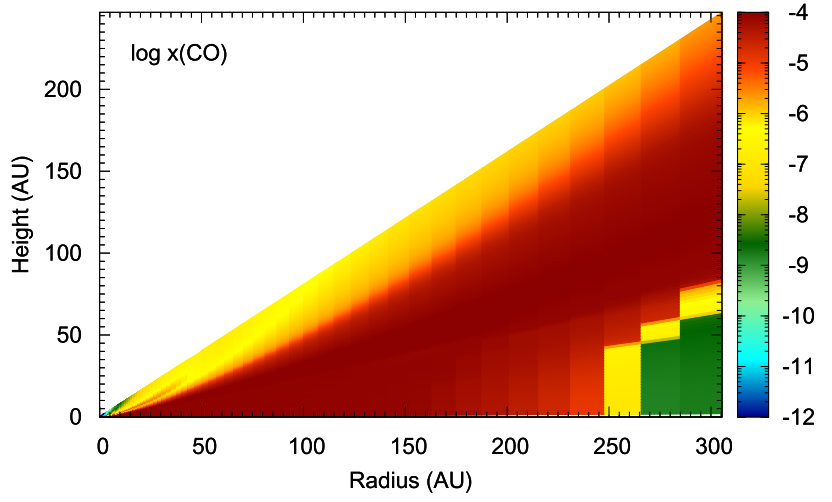
\includegraphics[width=0.33\linewidth]{walsh10_Xco.png}}\hfill%
  \subcaptionbox{\hco abundances}{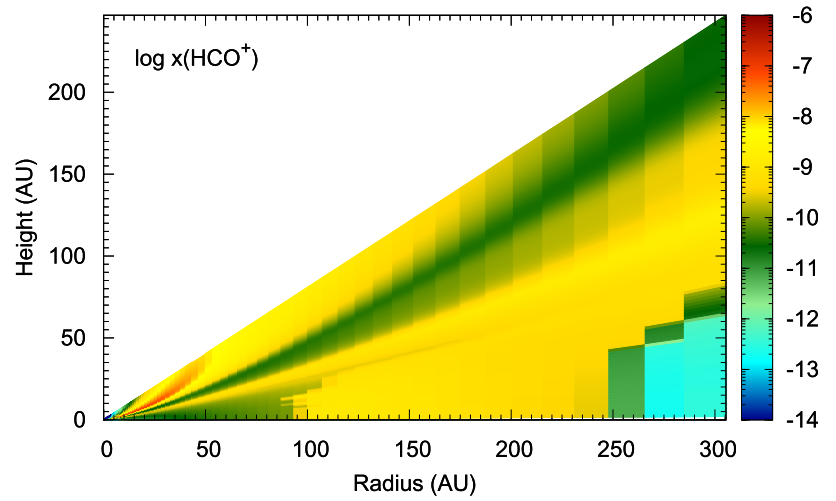
\includegraphics[width=0.33\linewidth]{walsh10_Xhco.png}}%
  \subcaptionbox{HCN abundances}{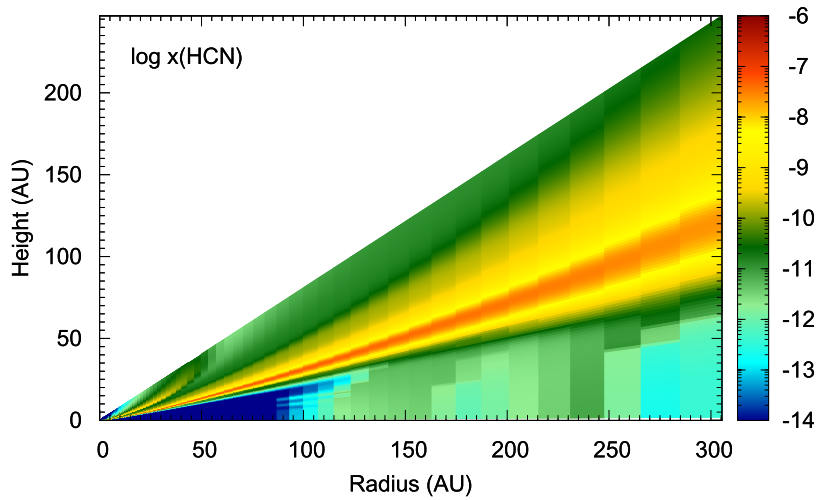
\includegraphics[width=0.33\linewidth]{walsh10_Xhcn.png}}%
  \hspace*{\fill}%
  \caption{Models from \citet{Walsh2013} showing radial and vertical distributions of CO, \hco, and HCN in a simulated disk around a T-Tauri star, being radiated by a nearby O star.}
  \label{fig:walsh-abundance-profs}
\end{figure}


\textit{Why does sam keep referencing Walsh2013 (which includes ionization) instead of Walsh2010, which is for an isolated disk?}



% Walsh et al. (2013) modeled the structure and emission from a disk surrounding a T Tauri star, being irradiated by a nearby O star and compared the gas line emission to that from an isolated disk. They found that, in general, line emission from the irradiated disk showed higher peak values due to the warmer disk. This was not the case for HCO+ which traces the cold, dense areas of the disk. Thus, the ratio of the HCN/HCO+ peak intensities can be used to roughly characterize the level of external irradiation, with HCN/HCO+ > 1 indicating an irradiated disk and HCN/HCO+ < 1 characteristic of an isolated disk.




\citet{Miotello2017} showed using isotopologues of CO that disks in Lupus have gas/dust ratios far below the literature value of 100, instead indicating that values of order 10 or even 1 are more appropriate. This was echoed by

Compare to slide 8/11 here:
https://www.cv.nrao.edu/rocks/pdf/S2-P4_rocks2013_millar.pdf


Good overview:
https://arxiv.org/pdf/1901.10862.pdf

Williams and Best: 100:1 is too high.
https://iopscience.iop.org/article/10.1088/0004-637X/788/1/59/pdf

Really good(-looking) paper on gas/dust ratio/chem models:
https://www.aanda.org/articles/aa/pdf/2017/03/aa29556-16.pdf




\section{Planet-Forming Potential}
\label{section:fitting_procedure}

In order to gauage a disk's planet forming potential, we may begin by referring to the MMSN

One way to contextualize the results presented in \S\ref{chap:analysis} is through the lens of planet formation. This analysis traditionally begins with a comparison to the MMSN, which is the density profile that our own Solar System would have if all our planets had gas added to them until their composition matched that of the Sun, then each planet's mass was spread out in a ring along its orbital path (as discussed in \S\ref{chap:introduction}). Integrating this mass leaves us with $M_\text{MMSN} \approx 0.01 M_\odot$. It is worth reiterating that this is an extremely rough metric, build on several assumptions, and that it does not reflect \textit{minimum} mass of a planet forming potential, but rather an approximation of the mass it would take for a disk like ours to form.

With the extremely large mass of $M = 0.36M_\odot$ that we measure in the CO line, it is needless to say that the disk's mass would not be its limiting factor in planet formation.





\section{Best Fit Temperature }
\label{section:fitting_procedure}

We begin by comparing to \citet{Factor2017}, in which they used similar methods of analysis to characterize another ONC proplyd, drawn from the same survey as our binary. Their results are presented in \ref{table:factor_fits}.


\begin{table}
  \centering
  \begin{threeparttable}
    \caption{Best-fit Results from \citet{Factor2017}}
    \label{table:factor_fits}
    \renewcommand{\arraystretch}{1.2}
    \begin{tabular}{l c c c c c }
      \toprule \toprule
      %\multirow{2}{*}{Parameter} & \multirow{2}{*}{Disk A}    & \multicolumn{2}{c}{Disk B} \\
      \multirow{2}{*}{Parameter} & \hco (thesis) & \hco (paper)  & HCN    & CO    & \hco \& CO \\
      \midrule %\midrule
      q                          & -0.02         & 0.17          & -0.18  & -0.33 & -0.24       \\
      T$_\text{atms}$ (\si{\K})  & 22            & 190           & 19     & 70    & 86          \\
      X$_\text{mol}$             & [-10]         & -10.07        & -6.7   & [-4]  & -10.04, [-4] \\
      \bottomrule
    \end{tabular}
    \begin{tablenotes}\footnotesize
      \item[*] CO values are from Sams paper. In his thesis, CO vals are [-0.3, 41, [-4]].
    \end{tablenotes}
  \end{threeparttable}
\end{table}

Comparing our results for disk A to theirs, we can see that our atmospheric temperature for the \hco fit is fairly well-aligned with their result. However, while our HCN fit is in quite close agreement with that of \hco, it is significantly higher than what they found.

Additionally, their temperature structures are systematically negative save for in the \hco line, where it is marginally positive. Ours, conversely, are systematically positive, and relatively larger than theirs. I don't know what to make of this\footnote{It also strikes me as strange that my temperatures are higher, since disk A's abundances for HCO+ are >two OoM higher than Sam's.}.


For the disk B fit, temperatures were notably higher across all lines, falling in the low 200's\footnote{Since the disk was not resolved, we were unable to fit for its temperature structure exponent, and thus fit it at -0.5 for all lines.}. Since


It is (maybe?) possible that this reflects the fact that our fits had different values for some of the fixed parameters. These include R$_{crit}$, which we fix at 100 and they fixed at 600 AU, as well as $z_q$ and $T_\text{mid}$, which they fit for and which together control how the temperature structure decays vertically (see \S\ref{subsection:physical_profs} for a more complete description). Since they fit multiple lines simultaneously, they were able to constrain these parameters, which is not possible in the case of single-line fitting. In a CO and \hco fit, they found values of $z_{q, 150} = 73$ AU and T$_{mid} = 24.7$ K, in comparison to our values of 29 and 19, respectively. \textit{Is this enough to make an appreciable difference? I don't know. It seems most likely to me that those drastically different R$_C$ values could explain the different q values, since if my disks are having their densities killed way earlier, then maybe they're struggling to match the flux levels further out. }

\textit{Another question about Sam's work: His paper and thesis have different values for the \hco and CO fits. He also makes no mention of the multi-line fits in his paper, which seems weird.}


% The expected value for q in a geometrically flat, optically thin disk is -0.5 while measured values vary from -0.6 to -0.3 (Dartois et al. 2003; Rosenfeld et al. 2012a,b)






\section{HCO$^+$, HCN Abundance Structures}
\label{section:fitting_procedure}










% The End
